%\documentclass[10pt]{beamer} % 4/3 aspect ration works as well
\documentclass[10pt,aspectratio=169]{beamer}
%----------------------------------------------------------------------------------------
%	PACKAGES AND THEMES
%----------------------------------------------------------------------------------------

\mode<presentation>{
  \usetheme{EuXFEL}
  \usecolortheme{EuXFEL}
}
\usepackage{hyperref}
\usepackage{amsmath}
\usepackage{graphicx}
\usepackage{subfigure}
\usepackage{xcolor}
\usepackage{colortbl}
\usepackage{helvet}
\usepackage[font=normalsize,labelfont={bf}]{caption}
\usepackage[T1]{fontenc}
\usepackage{tikz}
\usetikzlibrary{shapes, arrows, calc, positioning}
\usetikzlibrary{decorations.pathreplacing}
\usepackage{amsmath,amssymb}%,amsthm,amsxtra,mathabx}
\usepackage{lipsum}
\usepackage{verbatim}
\usepackage{datetime}
\usepackage{tcolorbox}
\usepackage[authordate,bibencoding=auto,backend=biber,natbib,doi=false,isbn=false,url=false,eprint=false]{biblatex-chicago}
\addbibresource{ref.bib}

\newcommand{\nb}[1]{{\color{gray} {#1}}}
\newcommand{\nblue}[1]{{\color{ceruleanblue} {#1}}}

\renewcommand{\familydefault}{\sfdefault}
\renewcommand\mathfamilydefault{}
\newcommand{\colorbf}[1]{{\color{xOrange}\textbf{#1}}}
\definecolor{burntorange}{rgb}{0.8, 0.33, 0.0}
\definecolor{ceruleanblue}{rgb}{0.16, 0.32, 0.75}
% Define custom style for the quote box

\tcbset{
  quotestyle/.style={
    colback=white,
    colframe=white,
    boxrule=0pt,
    arc=0pt,
    left=5cm,
    right=0cm,
    top=0.5cm,
    bottom=0.5cm,
    enhanced,
    sharp corners,
    width=\textwidth,
    fontupper=\fontsize{13}{17}\selectfont\color{burntorange!70},
  }
}
\newdateformat{dmydate}{%
    \twodigit{\THEDAY}~\monthname[\THEMONTH] \THEYEAR
%    \dayofweekname{\THEDAY}{\THEMONTH}{\THEYEAR} \twodigit{\THEDAY}~\monthname[\THEMONTH] \THEYEAR      
}   

\title[LLMs in Public Opinion Research]{Leveraging AI \& LLMs for Richer Insights into Public Opinion: Applications and Opportunities}

\author{Dr. Zachary P Dickson} % Your name
\institute[LSE] % Your institution as it will appear on the bottom of every slide, may be shorthand to save space
{\noindent
  \texttt{\color{purple}z.dickson@lse.ac.uk}\\% Your email address
  \href{https://z-dickson.github.io/}{\color{blue}https://z-dickson.github.io/}\\
  Research Fellow in Quantitative Methods\\
  Research Affiliate at the LSE Data Science Institute
  
}
\date{May 2025} % Date, can be changed to a custom date

\setbeamersize{text margin left=.05\pdfpagewidth,text margin right=.05\pdfpagewidth}

%\vfill
%
\includegraphics[scale=0.55,keepaspectratio]{desy_logo.pdf}


\begin{document}

%{
%  \setbeamertemplate{headline}{}
%  \begin{frame}
%    \titlepage
%   \end{frame}
%}
{
  \setbeamertemplate{headline}{}
  \begin{frame}
    \titlepage
    \vspace{-0.8cm}
    \hbox{
    
\includegraphics[scale=0.03,keepaspectratio]{figures/London_school_of_economics_logo_with_name.jpg}
      %
\includegraphics[scale=0.2,keepaspectratio]{figures/dept_of_methodology.png}
      %
\includegraphics[scale=0.05,keepaspectratio]{figures/LSE_DSI.png}
    }
  \end{frame}
}

\AtBeginSection[]
%{
%    \begin{frame}
%        \frametitle{Overview}
%        \tableofcontents[currentsection]
%    \end{frame}
%}





%\begin{frame}{The populist right has increasingly politicised Net Zero}

%\begin{columns}[onlytextwidth]
%    \begin{column}{0.4\textwidth}

%\begin{figure}[H]
%\centering
%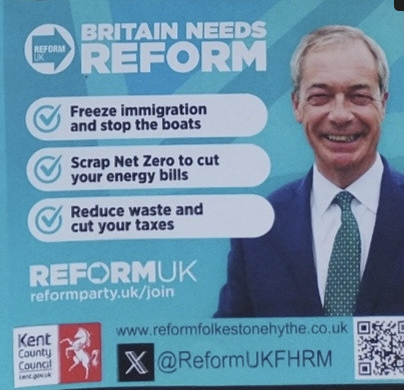
\includegraphics[scale=0.32,keepaspectratio]{figures/reform_2025.png}
%\caption{2025 Reform UK leaflet}
%\end{figure}

%\bigskip 
%\bigskip 

%\end{column}
%\begin{column}{0.6\textwidth}

%\begin{figure}[H]
%\centering
%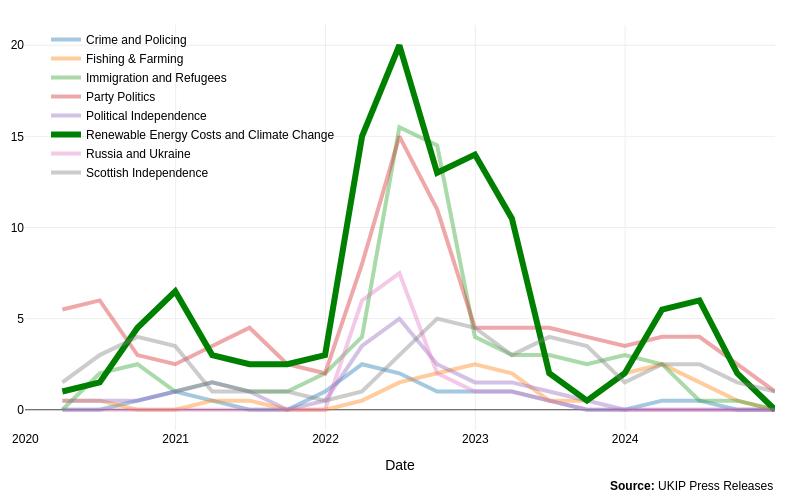
\includegraphics[scale=0.28,keepaspectratio]{figures/ukip_dynamic_topic_model_QE_rolling2.png}
%\caption{Dynamic topic model of UKIP press releases}
%\end{figure}

%\bigskip \bigskip 


%\end{column}
%\end{columns}

%\end{frame}







\section{Language Models and Public Opinion Research}

\begin{frame}{Language Models and Public Opinion Research}

\begin{itemize}
    \item LLMs can't replace a high quality opinion survey (\textit{yet})
    \begin{itemize}
        \item Representativeness 
        \item Variance in responses 
    \end{itemize}
    \item LLMs are a powerful complement to measuring opinions and behaviour 
    \item Exciting pathways for LLMs in survey research:
    \begin{itemize}
        \item Dynamic/adaptive surveys and interviews
        \item Generate/simulate new survey data* 
        \end{itemize}
\end{itemize}
\end{frame}



\begin{frame}{LLMs in [Adaptive] Survey Research}


\begin{itemize}
    \item Dynamic/adaptive surveys with embedded LLMs \textcolor{gray}{\small \citep{velez2024confronting}}
    \begin{itemize}
        \item Survey questions can be translated or modified to reflect user input  
    \end{itemize}
    \item Conversational surveys via interview \textcolor{gray}{\small \citep{geiecke2024conversations}} 
    \begin{itemize}
        \item AI-led qualitative interviews at scale 
    \end{itemize}
\end{itemize}    

\begin{tcolorbox}[quotestyle]
        \textit{``AI-powered interviewers can create a\\ bridge between the richness of qualitative\\ data and the statistical power of quantitative data'' (Geicke \& Jaravel, 2024)}
    \end{tcolorbox}

\end{frame}





\begin{frame}{Language Models in Interviewing for Electoral Choices}
	
	\begin{center}
		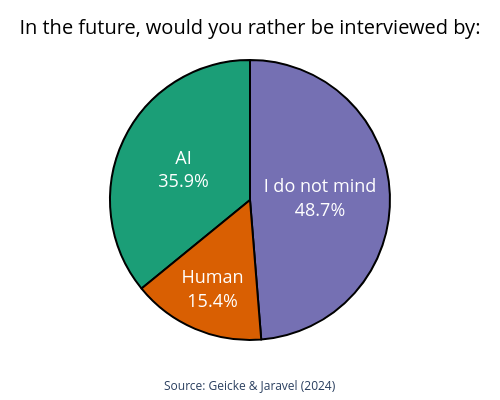
\includegraphics[width=.5\textwidth]{figures/piechart.png}
\end{center}
\end{frame}







\begin{frame}{Dynamic/Adaptive Surveys}

\nblue{\citet{velez2024confronting}}

\begin{center}
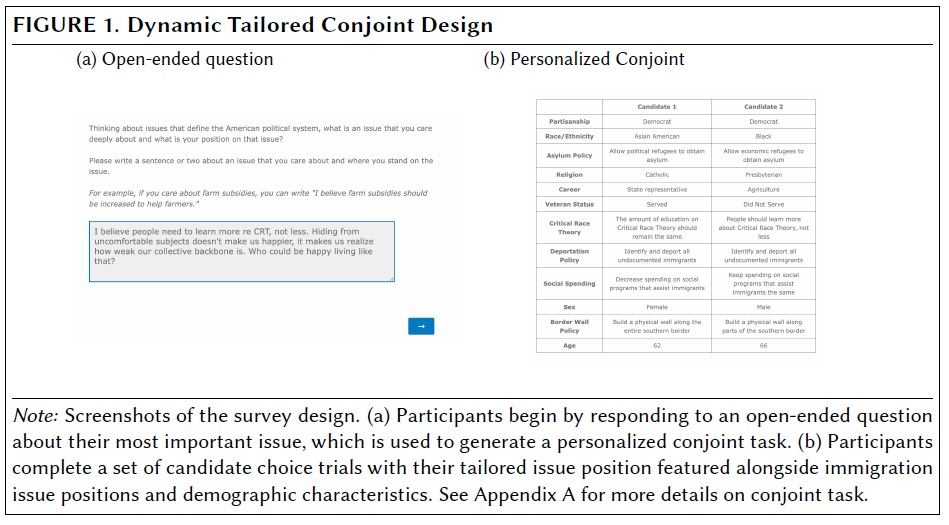
\includegraphics[width=.6\textwidth]{figures/velez_conjoint.jpg}
\end{center}

\end{frame}












\begin{frame}{Synthetic Data Generation with LLMs}

\textbf{Examples:} \medskip 
	\begin{itemize}
	\item Simulated human samples \nb{(Argyle et al 2023) } \medskip 
	\begin{itemize}
		\item Questionable reliability \nb{(Bisbee et al 2023)} 
	\end{itemize}
	
	\medskip
	\item Behavioural game theory applications \nb{(Li et al 2023; Akata et al 2023)}
	
	\medskip
		\item Simulated social media environment (using LLMs to interact w/ respondents) \nb{(Allamong et al 2024)}
			\medskip
		\item LLM performance in wargames \nb{(Lamparth et al 2024)}
		\medskip
		\item Do humans or LLMs make more convincing political arguments? \nb{(Palmer \& Spirling 2024)}
	\end{itemize}
\end{frame}
















\begin{frame}{Simulating Public Opinion with LLMs}

	\nblue{Bisbee et al (2024)}
	\begin{center}
		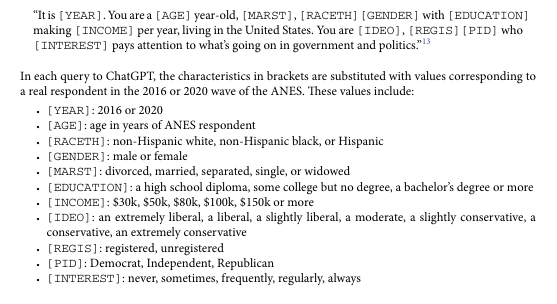
\includegraphics[width=.7\textwidth]{figures/bisbee_prompt.png}
	\end{center}
\end{frame}



\begin{frame}{Can LLMs Represent Public Opinion?}
	\nblue{Bisbee et al (2024)}
	\begin{center}
		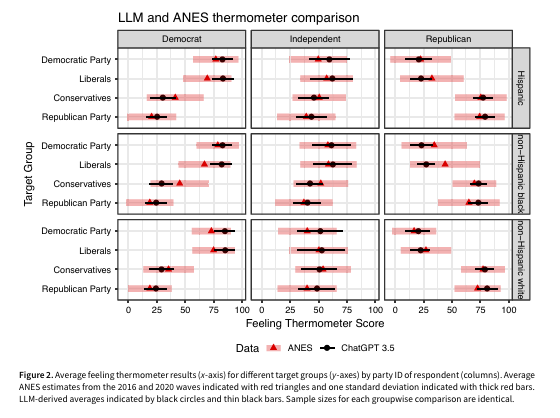
\includegraphics[width=.6\textwidth]{figures/bisbee_results.png}
	\end{center}

\end{frame}








\begin{frame}{The Path Forward: Opportunities \& Responsible Innovation}

\begin{itemize}
    \item Opportunities
    \begin{itemize}
        \item New insights from combining diverse data
        \begin{itemize}
            \item Adaptive and dynamic surveys 
            \item Synthetic data*
            \item Improving existing surveys (wording, cultural sensitivity etc.)
        \end{itemize}
    \end{itemize}
    \item Key Challenges \& Considerations
    \begin{itemize}
        \item Ethics: Privacy, potential for misuse (e.g., microtargeting, manipulation -- \href{https://www.reddit.com/r/changemyview/comments/1k8b2hj/comment/mp4vgcm/?share_id=W7n2eWmaRZq3odRwfc_-5}{Reddit story})
        \item Validation: very early days for LLMs -- be curious, but be caution and consult a range of experts outside your domain
    \end{itemize}
\end{itemize}


\end{frame}




\begin{frame}{}

\bigskip 

\textbf{\Large Thank you for your attention!}
\bigskip 


    
\end{frame}











\begin{frame}{Enhancing Surveys with LLMs}
\begin{itemize}
    \item \textbf{Complementing existing survey methods }
    \begin{itemize}
        \item Improving question wording \textcolor{gray}{\citep{wang2024autosurvey}}  
        \item Questionnaire pretesting in cross-cultural settings \textcolor{gray}{\citep{adhikari2025exploring}}
        \item Analyzing open-ended questions/responses \textcolor{gray}{\citep{mellon2024ais}}
    \end{itemize} 
\end{itemize}
\end{frame}






\end{document}